\documentclass{article}
\usepackage[utf8]{inputenc}
\usepackage{graphicx}
\usepackage{float}


\graphicspath{}


\title{Allometric Modeling and Dimensional Analysis}
\author{Geneva Porter}
\date{13 September 2018}

\begin{document}
	
\begin{titlepage}
\maketitle
\vspace{10mm}


\centering
\large \it San Diego State University

Professor Mahaffy, Math 636
\end{titlepage}

\section{Kepler's Third Law}

This problem investigates planets of the Solar System and  the relationship between their distance from the sun and the length of their revolution period around the sun. Data from the Jet Propulsion Laboratory was used to generate the models. The figures use units of $10^6km$ for distance and earth days for revolution period.

Examining Figure 1, we see a power model matching the data given. The power model is given in the form $p=kd^a$, with $p$ equal to the revolution period, $d$ equal to the distance from the sun, and $k$ and $a$ are constants. Using Matlab, the values of $k$ and $a$ were calculated as $0.199$ and $1.50$, respectively.We can see that the data matches the model fairly well with data from Mercury, Earth, Jupiter, and Mars, and would likely provide accurate predictions of other planets.

\begin{figure}[H]
	\centering{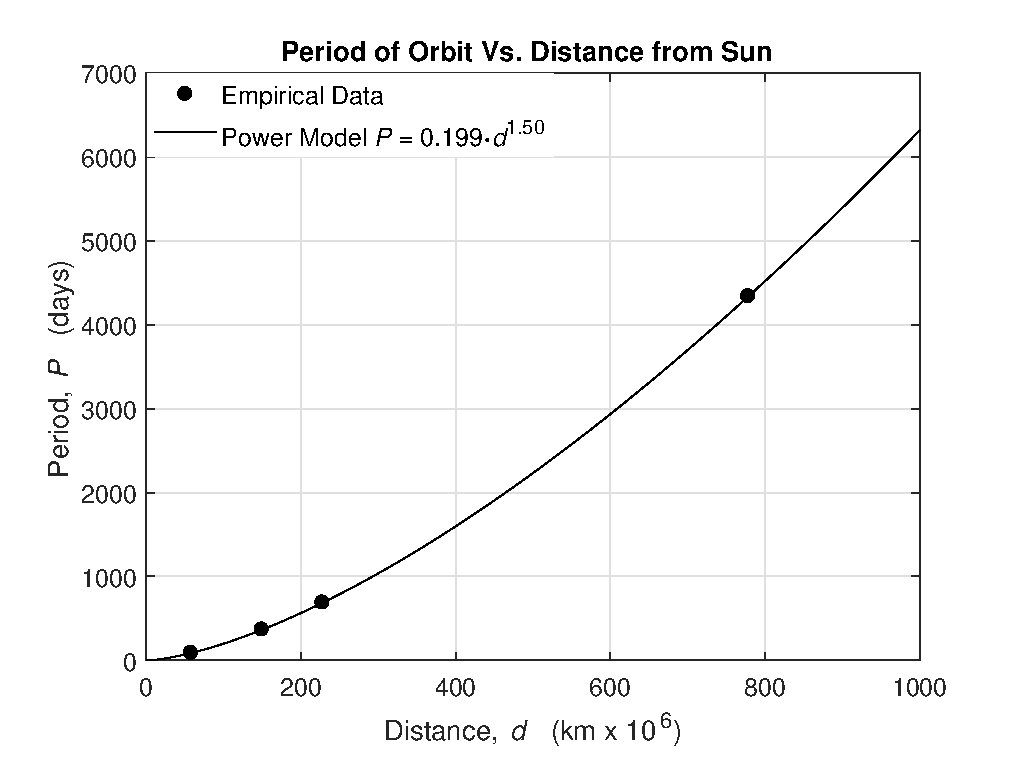
\includegraphics[width=10cm]{powerPvD.eps}}
	\caption{P vs. d}
\end{figure}

Figure 2 (next page) also shows the data points, however they are shown against a logarithmic model. To accomplish this, first it is necessary to take the natural log of each datum point. Doing this will show that this set of data models a straight line. To find the equation of this line, our values of $k$ and $a$ are used again:

\vspace{5mm}  

\centerline{$p=kd^a \rightarrow log(p)=log(kd^a) \rightarrow log(p)=log(k)+a\cdot log(d)$}

\pagebreak

Now we have an equation in the form of $y=b+mx$. In this case the slope is $a$ and the intercept is $log(k)$. Both graphs model the data accurately, and the logarithmic model can also be used to find the constants for the power model (rather than our method of finding the power model first).


\begin{figure}[H]
	\centering{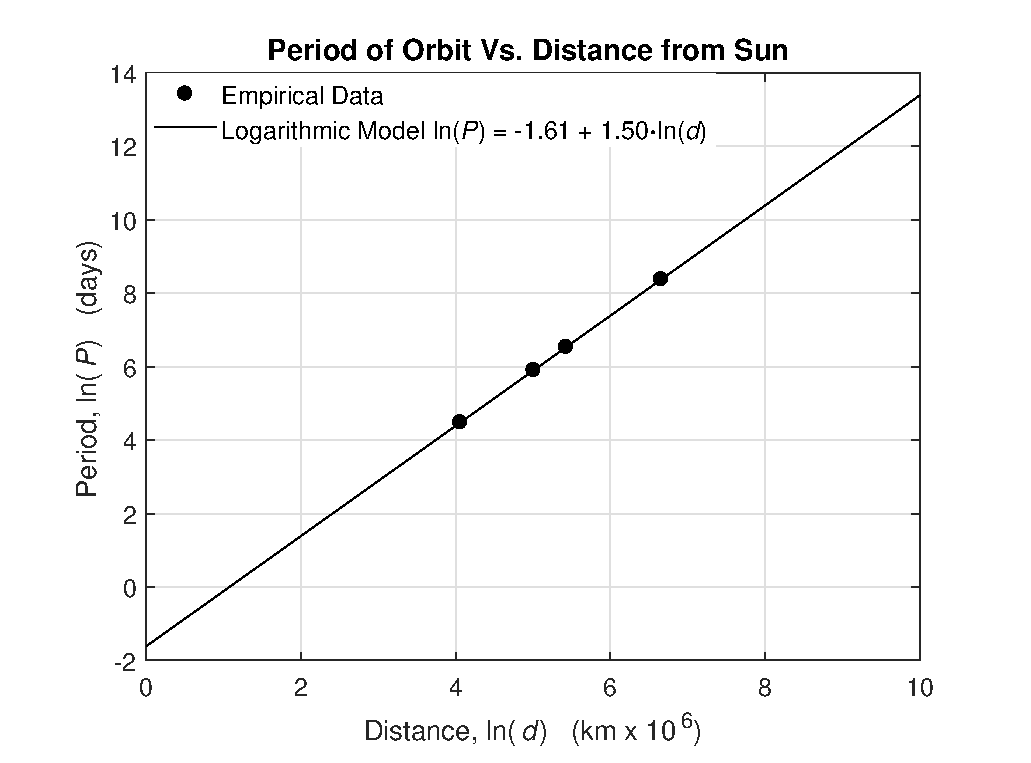
\includegraphics[width=10cm]{logPvD.eps}}
	\caption{ln(P) vs. ln(d)}
\end{figure}

Using the measurements from the Jet Propulsion Laboratory, we can calculate how accurate the model is. For the Planets Venus, Uranus, and Neptune, the sum of squared errors for the predicted period versus the observed period is 6,226. Considering that this data deals in large-scale behavior, this sum would not be considered a large error. Also, for the planets Saturn and Neptune, the sum of the squared errors of the predicted distance from the sun and the observed distance from the sun is $2.0355\cdot 10^{18}$. Note that these units are in $10^6km$, so this figure seems rather large. However, this model would still be considered successful with a rough measure of accuracy.

Using dimensional analysis, we can also see that the power model has the correct values. Kepler's third law stated that the square of the orbital period of a planet is directly proportional to the cube of the semi-major axis of orbit. When evaluating the period ($p$), we must not only consider the planet's distance from the sun ($d$) but also consider the force of gravity ($F_g$) and the centripetal force ($F_c$). To set up our dimensional analysis, we start here:

\pagebreak

$p=[T],$ $ d=[1/(2\pi)\cdot L],$ $ F_g=[GM\cdot M\cdot L^{-2}]$, and $F_c=[M\cdot L\cdot T^{-2}]$

\vspace{5mm}

We can omit the constants $1/(2\pi)$ and $GM$, leaving us with:

\vspace{5mm}

$\Pi=[p]^a\cdot [d]^b\cdot [F_g]^c\cdot[F_c]^d$, where

\vspace{5mm}

$a=2,$ $ b=-3, $ $c=-1,$ and $d=1$ so

\vspace{5mm}

$\Pi=p^2\cdot d^{-3}\cdot F_g^{-1}cdot\ F_c^{1}=k$

\vspace{5mm}

Solving for period $p$, we get:

\vspace{5mm}

$p^2=d^3\cdot F_g/F_c\cdot k$, or $p=d^{3/2}\cdot (F_g/F_c)^{1/2}\cdot k$

\vspace{5mm}

Which shows that our exponent of $\approx$1.50 is close to the true value.



\pagebreak

\section{Biodiversity}

This problem focused on the relationship between island land mass and the population of amphibians and reptiles, called herpetofauna. The number of species were measured over areas in $km^2$.

In Figure 3 below, a power model was fitted to 5 data pairs of land area and number of species. We can see that the data fits in a general way, but for islands smaller than $2\cdot 10^4 km^2$ it is difficult to visually discern the differences in species presence.

\begin{figure}[H]
	\centering{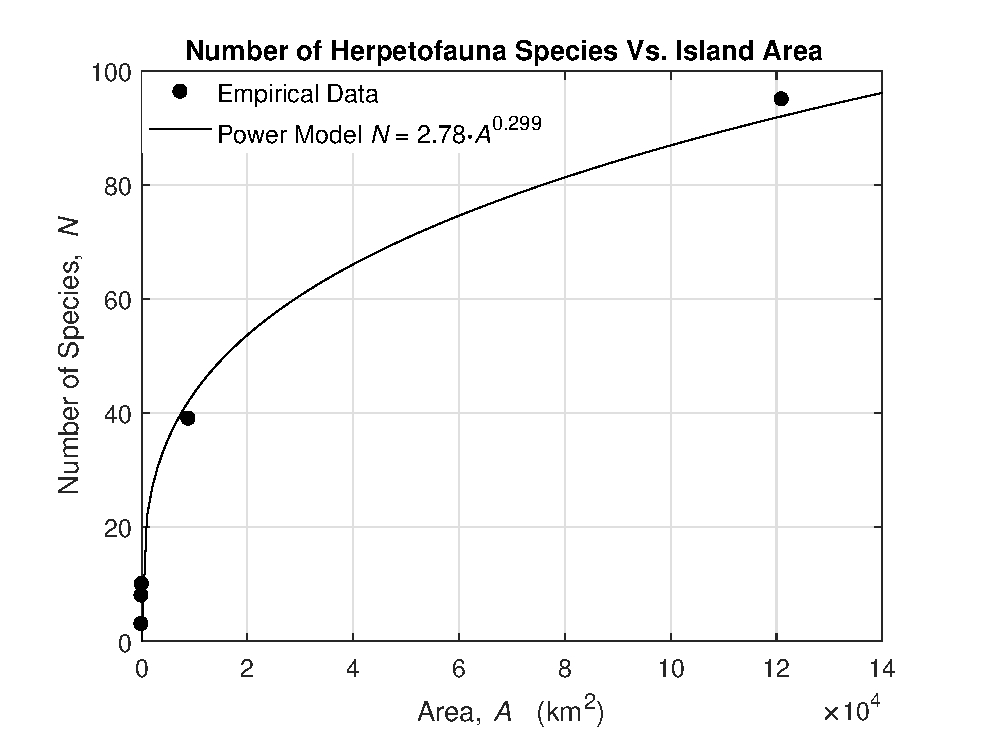
\includegraphics[width=10cm]{powerNvA.eps}}
	\caption{N vs. A}
\end{figure}

Examining Figure 4 (next page), we can see more clearly how well the data fit the model. Here we have a logarithmic model, created using the same method as in Problem 1. The power model

\vspace{5mm} 

$N=K\cdot A^m$ 

\vspace{5mm}

was used to form the logarithmic model

\vspace{5mm} 

$log(N)=log(K)+m\cdot log(A)$. 

\vspace{5mm}

The parameter $m$ stays the same value in both models, and $K$ differs by taking the natural log for the logarithmic model (or the exponential, if you created the logarithmic model first).

These models suggest that there is an obvious correlation between land mass and biodiversity. Mitigation efforts by construction-related organizations may or may not be sufficient to sustain biodiversity. Many species are highly adapted to a small yet complex ecosystem, so extending this model to different regions on earth depends on logistic and political efforts. 

Mathematically speaking, when applied to land masses not contained in an island, such a model may have potential. When examining the biodiversity of larger mammals, surely the area needed increases significantly for the same number of species, particularly for predatory creatures. In this case the intercept parameter of the logistical model may differ only slightly, yet the slope parameter will surely increase a large amount. Conversely, for modeling very small species such as insects, we would expect the slope parameter to be closer to the herpetofauna model, as insects do not need relatively large areas of land to survive in large numbers. 

An interesting model to study would be the relationship between animals of different groups and how their size influences the amount of area they need to maintain their population (a biologist might point out that the relationship is actually visa versa).


\begin{figure}[H]
	\centering{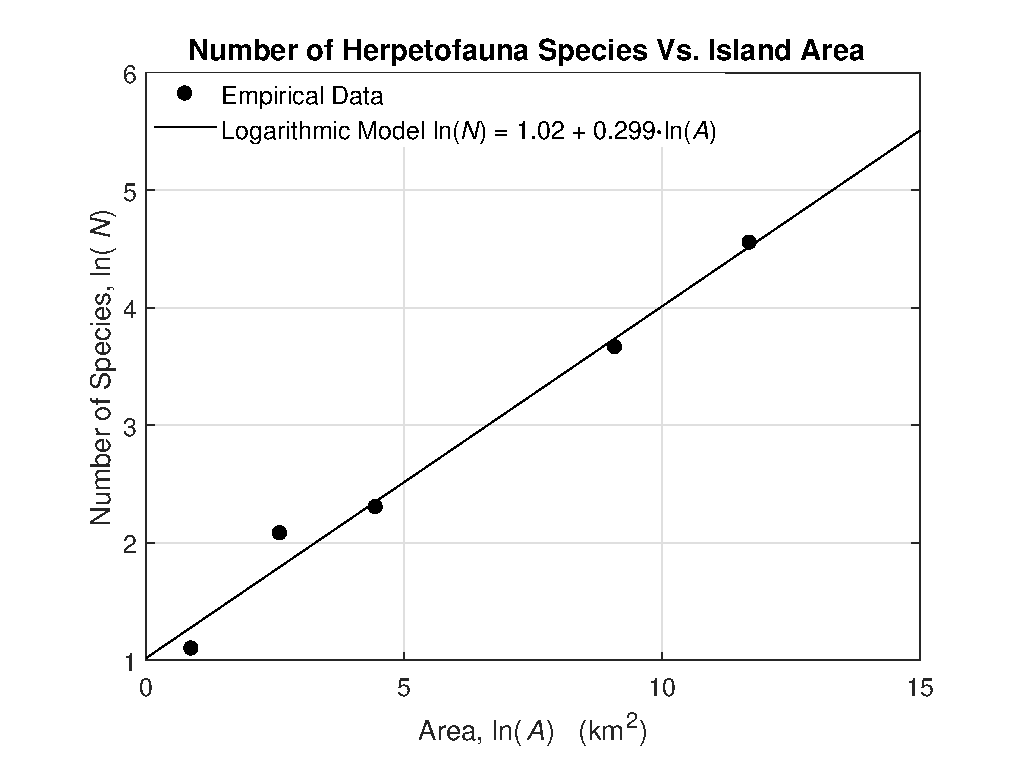
\includegraphics[width=10cm]{logNvA.eps}}
	\caption{ln(N) vs. ln(A)}
\end{figure}

\pagebreak

\section{Tree Volume}

Here we investigate the relationship between the diameter, height, and volume of trees in the Allegheny National Forest in Pennsylvania. The diameter of thew trees is measured in inches, the height in feet, and the volume in board feet (1 board foot would be equal to a square foot base with a height of 1 inch).

looking at figures 5 and 6, we can clearly see that the volume of a tree has a stronger correlation to its diameter than its height. This is logical, because young trees often gain height before girth, as an evolutionary mechanism to reach more sunlight above the brush layer of a forest. In this case the tree may have gained a significant amount of height before gaining volume. The diameter, on the other hand, can indicate not only how tall the tree is but how old it is as well. Concentric rings mark the passing years on trees that have fallen, and modeling more data would show the relationship between tree age and diameter clearly.


\begin{figure}[H]
	\centering{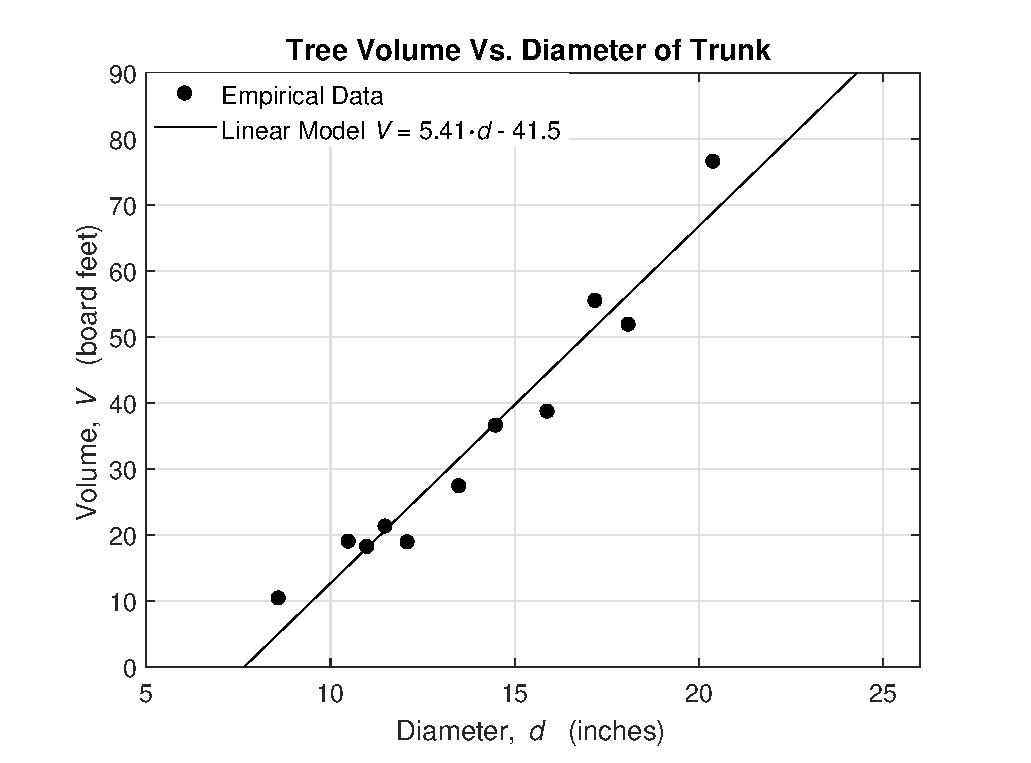
\includegraphics[width=10cm]{linearVvD.eps}}
	\caption{V vs. d}
\end{figure}


From the models we can also see that the intercepts for both are negative, indicating that the volume would be less than zero for trees with diameters less than 7 inches or trees with heights less than 50 inches. Of course, when modeling real-world relationships, negative values are excluded. Since there was no data included for trees with relatively small volumes such as saplings, we cannot predict heights or diameters for volumes close to zero. If that data were included, then the model would probably not fit a linear curve well.

\begin{figure}[H]
	\centering{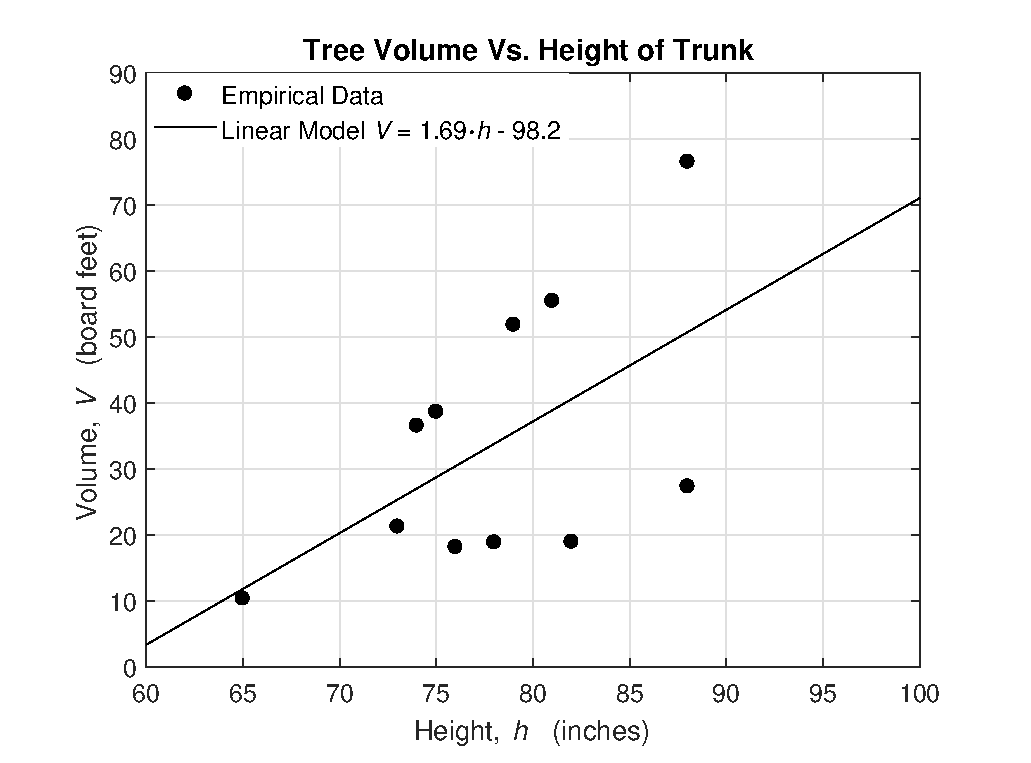
\includegraphics[width=10cm]{linearVvH.eps}}
	\caption{V vs. h}
\end{figure}

Below in Figure 7, a power model was used. We can see that the y-intercept is more realistically near 0. Parameters $K$ and $A$ were used as the coefficient and the power, respectively. The value of $A$ is about 2, meaning that the volume of a tree is proportional to its diameter squared. This is logical, as the volume of a cylinder has a similar relationship.

\begin{figure}[H]
	\centering{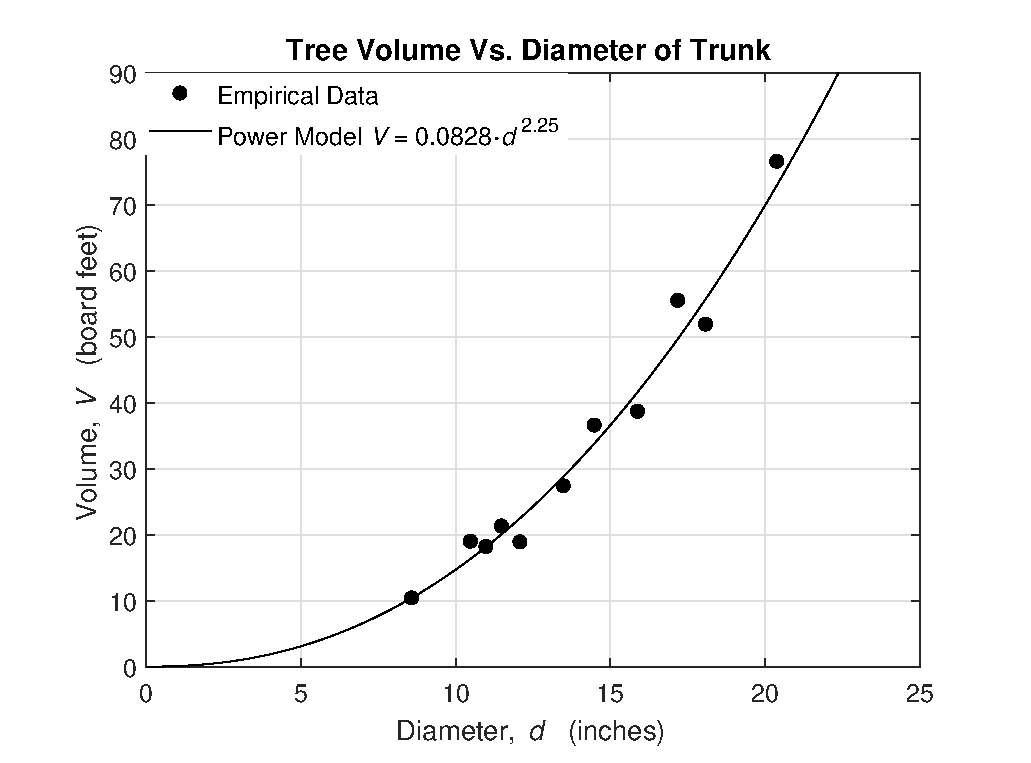
\includegraphics[width=10cm]{powerVvD.eps}}
	\caption{V vs. d}
\end{figure}



\section*{Male Kittens}

This problem discussed the relationship between a male kitten's weight, age, and food needs. First, data for weight and age were given, allowing the creation of an equation for weight as a function of age $W(t)$. Next, data for weight and food were give, producing a model based on food as a function of weight $C(W)$. Finally, a composite function was formed for food as a function of age, $C(W(t))$.

In the following figures, each function is modeled. While Figure 8 was fitted using a pre-existing function type, Figure 9 fitted the data straight to a power model.

 
\begin{figure}[H]
	\centering{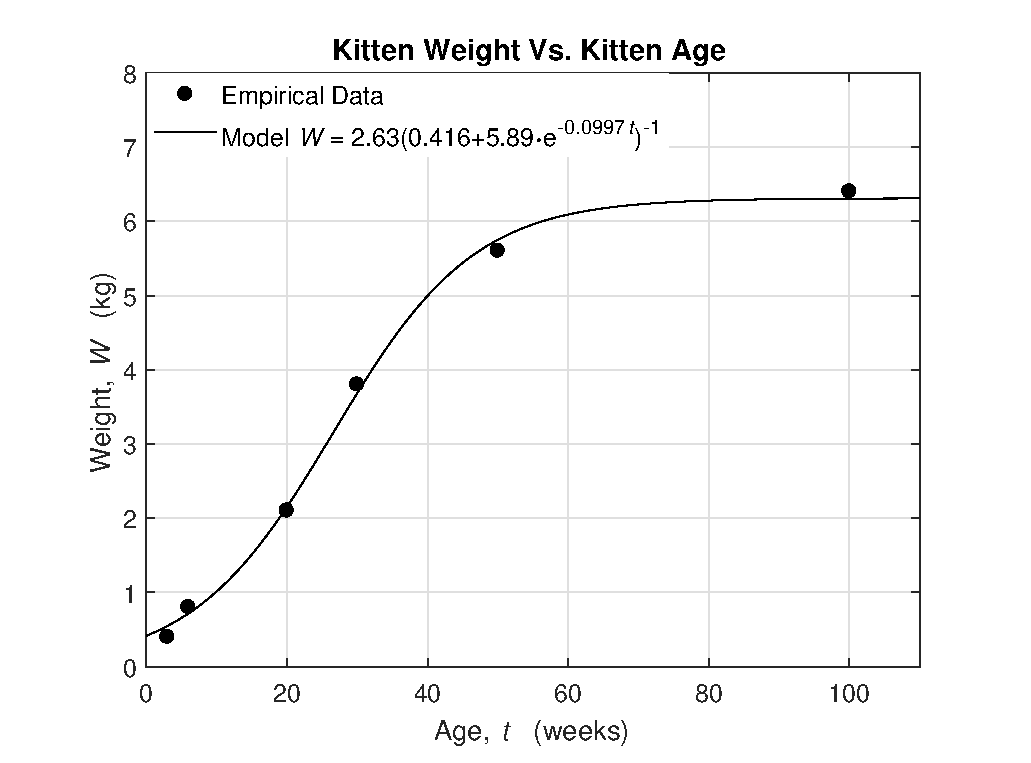
\includegraphics[width=10cm]{expWvT.eps}}
	\caption{W vs. t}
\end{figure}

For Figure 9, We can see the data fits quite well with a coefficient of 48 and a power of 0.7. We notice that this power is less than 1, which alludes to the correlation between growth rate and food. kittens gain weight relative to their current body size quickly at first, but more slowly as they age. We know that young mammals generally need a high calorie diet to accommodate body growth and energy expenditure, however both of these processes slow down after a certain point in time. 

Figure 10 displays our composite function. It has a noticeable feature of being quite similar to Figure 8. It also has an inflection point at $t=23$ weeks.This indicates that before this point, the rate of food consumption was increasing. After 23 weeks, the rate of food consumption decreases. 

\begin{figure}[H]
	\centering{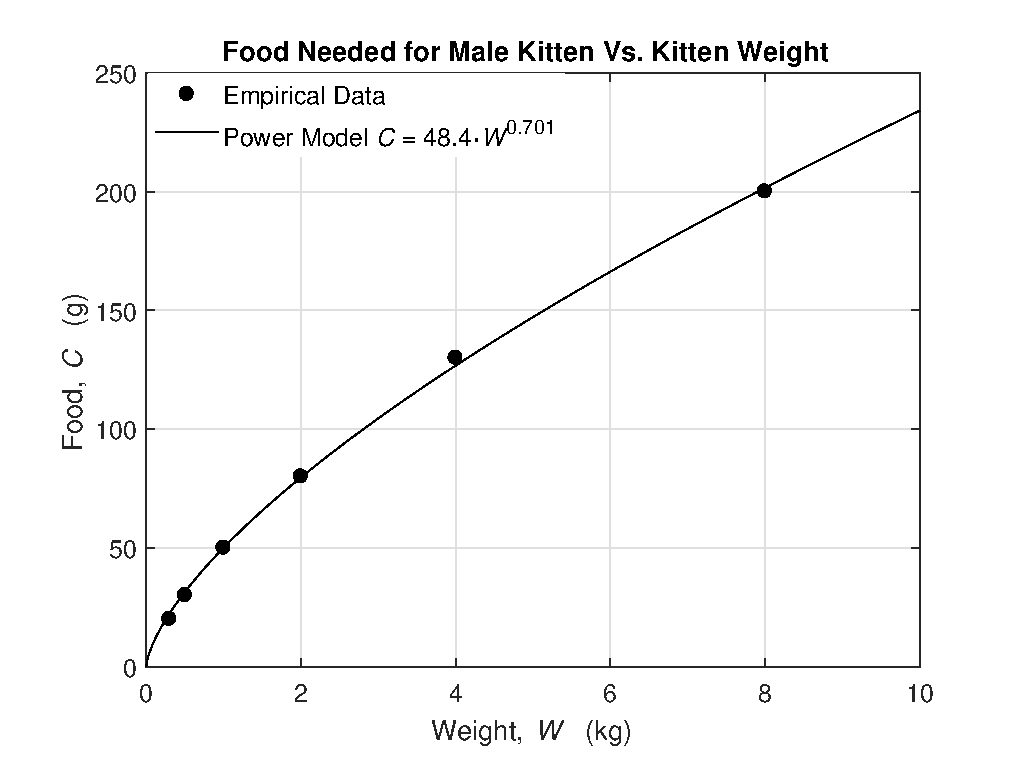
\includegraphics[width=10cm]{powerCvW.eps}}
	\caption{C vs. W}
\end{figure}


\begin{figure}[H]
	\centering{\includegraphics[width=10cm]{Cvt.eps}}
	\caption{C vs. t}
\end{figure}

\section*{Gulliver's Travels}

The well known tale of Gulliver still enchants children today. In it, he shipwrecks on an island, waking up surrounded by tiny people. These people, the Lilliputians, decided to feed Gulliver 1,728 times as much food as they feed themselves. They calculated Gulliver's height as 12 times their own, and thus would feed him $12^3$ times more than they would eat.

Let's assume that the Lilliputian's calculations are accurate, and the height of a Lilliputian is represented by $l$. Gulliver would then have a volume of $1728\cdot l^3$. Due to the non-linear relationship between mass and metabolic rate, Gulliver would not need this much food. 

Suppose that Gulliver's metabolism allows him to only loose energy through the skin. If we use an Allometric model to describe this energy loss, it will have the form $y=A\cdot x^r$, with $x$ being the weight of the subject. If we take Gulliver's total heat produced by volume ($l^3$) and compare it to his heat lost by area ($l^2$), we can say that Gulliver only needs $l^{2/3}$ the amount of food as a Lilliputian. They would only need to give him $(12^3)^{2/3}=144$ the amount of food they eat themselves. 

Kleiber's Law states that this exponent should in fact be 3/4, not 2/3. The larger number attests to the fact that the metabolic rate of animals is more complex than assumed. The rate of 3/4 comes from the logarithmic graph of Metabolic Rate vs. Weight, ($log(y)=3/4log(x)+log(k)$). the slop of that graph is 3/4, which is used for $r$ in the power model. Using this model, Gulliver would need $(12^3)^{3/4}=268$ times as much food as a Lilliputian.

\begin{figure}[H]
	\centering{\includegraphics[width=12cm]{gulliver.png}}
\end{figure}


\end{document}